\chapter{評価}
\label{chap:kekkahyouka}

\section{概要}
本論文の提案手法について評価するために, 次に示すの3つのRQを用意した. 

\begin{itemize}
  \item RQ1: レビューの抽出性能はどの程度か
  \item RQ2: クラスタリングの性能はどの程度か
  \item RQ3: 可視化ツールの有用性はどうか
\end{itemize}

RQ1では, BERTを用いた抽出モデルによるレビューの自動抽出性能について評価する. 評価する際は, モデルがレビューにキーフレーズがあるかどうかを正確に判断できるか, キーフレーズがある場合, そのキーフレーズを正確に抽出できるかという2点についてそれぞれ評価する. 

RQ2では, まず, 本研究のクラスタリング手法として使用したChinese Wispersで使用するグラフを決定するための適切な閾値について検証する. そして, Chinese Whispersのクラスタリング性能をK-Meansと階層型クラスタリングという2つのクラスタリング手法と比較して評価する. 

RQ3では, 本論文で実装した可視化ツールが開発者にとって有用なものあるかどうかを評価する. 一般的にレビューの閲覧や確認で使用されるGoogle Playストアのレビュー欄と比較することで, 本ツールの有用性を示す. 

\section{RQ1:レビューの抽出性能はどの程度か}
\subsection{評価方法}\label{method}
作成された抽出モデルの抽出性能について調査する. 使用するデータセットは\ref{dataset}項で先述したデータセット10,000件のうち, テストデータとした2,000件である. このテストデータの各レビューに対してキーフレーズの自動抽出を行い, 手動で抽出した正解データと比較した. 
この自動抽出に関しては, レビューにキーフレーズがないものはキーフレーズのない文章と判断し, レビューにキーフレーズがある場合はキーフレーズのある文章と判断する. また, キーフレーズのある文章に関してはレビューにある有用な情報をキーフレーズとする. 
キーフレーズがある文章では, 次に示す3つの場合に分けて評価する. 

\begin{itemize}
  \item 抽出したキーフレーズが完全に一致している場合
  \item 抽出したキーフレーズが部分的に一致している場合
  \item 抽出したキーフレーズが全く一致していない場合
\end{itemize}

\subsection{結果}
\ref{method}項の評価方法に基づいて検証された結果を表\ref{tb:qa}に示す. 

\begin{table}[H]
  \caption{kキーフレーズの抽出結果}
  \small
  \label{tb:qa}
  \begin{center}
  \begin{tabularx}{\linewidth}{X|r}
    \hline
    キーフレーズがある問題数&468\\\hline
    キーフレーズがある問題の正当数&261\\\hline
    キーフレーズがある問題の部分一致正答数&124\\\hline
    キーフレーズがない問題数&1532\\\hline
    キーフレーズがない問題の正答数&1483\\\hline\hline
    キーフレーズがある問題の正答率&55.8\%\\\hline
    キーフレーズがある問題の部分一致を含めた正答率&82.3\%\\\hline
    キーフレーズがない問題の正答率&96.8\%\\\hline\hline
    全体の正答率&87.2\%\\\hline
    部分一致を含めた全体の正答率&93.4\%\\\hline
  \end{tabularx}\end{center}
\end{table}

答えがない問題の正答率は96.8\%と非常に精度の高い結果となった. すなわち, 本研究で作成された抽出モデルはレビューにキーフレーズがあるかどうかを判別する精度が高いことが示された. 
一方で, 答えがある問題の正答率は55.8\%とあまり精度が高くないものの, 部分一致を含めた正答率は82.1\%と比較的高い結果が得られた. 

\subsection{考察}
正答率が下がってしまった原因に関して考察する. 
キーフレーズが存在する文章のうち誤って抽出してしまった例を表\ref{tb:mistake}に示す.

\begin{table}[H]
  \caption{ 正解データと自動抽出したキーフレーズが一致しない例 }
  \small
  \label{tb:mistake}
  \begin{center}
  \begin{tabularx}{\linewidth}{X|X|X}
    \hline
    元の文章&自動抽出したキーフレーズ&手動抽出したキーフレーズ\\\hline\hline
    店で使えずに仕方なく現金で払いました&&店で使えず\\\hline
    とにかく地図検索がクソ&とにかく地図検索がクソ&地図検索がクソ\\\hline
    急に曲が止まって何しても流れないから端末再起動させたらようやく流れた&急に曲が止まって何しても流れないから端末再起動させたらようやく流れた&急に曲が止まって何しても流れない\\\hline
    データのカウント数が減ることがある&データのカウント数が減る&カウント数が減ることがある\\\hline
    ウォーキングで設定してるのに10分の1しかカウントしない&ウォーキングで設定してるのに10分の1しかカウントしない&10分の1しかカウントしない\\\hline
    類似アプリと比べて突出した利点もなく、あえてlinemusicを選ぶ理由がない&&類似アプリと比べて突出した利点もなく\\\hline
    コークオンを使おうとしてるのに、使えないなんでか、解らない&コークオンを使おうとしてるのに、使えないなんでか&コークオンを使おうとしてるのに、使えない\\\hline
    12月1日正午再び開けなくなりバーコードのみ表示&再び開けなくなりバーコードのみ表示&開けなくなりバーコードのみ表示\\\hline
    クレジットカードがjcb縛りなんて驚愕です&&クレジットカードがjcb縛り\\\hline
    機内モードにすることで会員バーコードは表示できるのでチャージや支払いは出来るが、クーポンを取得したりできないので不便&クーポンを取得したりできない&機内モードにすることで会員バーコードは表示できるのでチャージや支払いは出来るが、クーポンを取得したりできないので不便\\\hline
  \end{tabularx}\end{center}
\end{table}

次にキーフレーズが存在しないレビューにも関わらず誤って抽出してしまった例を表\ref{tb:mistake2}に示す.

\begin{table}[H]
  \caption{ キーフレーズがない文章から誤って抽出した例 }
  \label{tb:mistake2}
  \begin{center}
  \begin{tabularx}{\linewidth}{X|X|X}
    \hline
    元の文章&自動抽出したキーフレーズ&手動抽出したキーフレーズ\\\hline\hline
    初めてはどきどきする&初めてはどきどきする&\\\hline
    wifiも4gも正常です&wifiも4gも正常です&\\\hline
    ふざけたアプリ&ふざけたアプリ&\\\hline
    改善策はあるのでしょうか&改善策はあるのでしょうか&\\\hline
    自分でインターネットで調べるまで、今回の不具合についての更新がある事を知りませんでした&不具合&\\\hline
    原因が分かりません、機種変してからか&原因が分かりません&\\\hline
    短いタイトルで読んでみたいと思うので、今後もわかりやすい記事を期待します&今後もわかりやすい記事を期待します&\\\hline
  \end{tabularx}\end{center}
\end{table}

このような結果から正答率の減少となる原因はいくつか考えられる. ここでは大きく分けて3つの原因を挙げる. 

1つ目は手動で抽出したキーフレーズの精度である. データセットは情報工学科の学部4年生の2名で作成したものだが, この2人の作成者はモバイルアプリに関する専門的な知識を持つ者ではない. そのため, 作成したデータセットの精度に問題があることが正答率の減少につながっていると考えられる. 
例えば, 表\ref{tb:mistake}にある``類似アプリと比べて突出した利点もなく、あえてlinemusicを選ぶ理由がない''というレビューに対して, 手動で``類似アプリと比べて突出した利点もなく''を抽出しているが, これはアプリの欠陥でもアプリに対する要望でもないため本来抽出するべきでない. 
また, 表\ref{tb:mistake2}にある``短いタイトルで読んでみたいと思うので、今後もわかりやすい記事を期待します''というレビューに対して, ``今後もわかりやすい記事を期待します''はアプリに対する要望にも関わらず, 手動では抽出していない. このように手動での抽出精度を上げることによって精度の向上が見られると考えられる. 

2つ目はレビューの特徴である. レビューは短く構造化されていないため, 内容が曖昧であったり, 意図が明確でなかったりするレビューが見受けられる. レビューは情報量が少ないものが多く, その記述がアプリに対する有用な情報なのかどうかを判断するのは難易度が高い. 
以上より, レビューの特徴が自動抽出の精度に大きな影響を与えていると考えられる. 

3つ目は本研究のタスクの難易度の高さである. 本研究のタスクは質問応答形式のタスクの中でも, キーフレーズが名詞や動詞などの1つのトークンだけではなく, 複数のトークンを含めることが多いため抽出する人や抽出モデルによって結果が変わる難易度の高いタスクである. 
したがって, 本研究における自動抽出タスクの難易度が高いことが正答率を減少させている大きな要因となっている. 

次に, 自動抽出したキーフレーズの特徴や傾向に関して考察する. 
自動抽出した結果と手動で抽出した結果を比較すると, 自動抽出した結果の方がキーフレーズを長めに抽出する傾向にあることがわかる. 
例えば, ``12月1日正午再び開けなくなりバーコードのみ表示''というレビューに対して, 自動抽出では``再び開けなくなりバーコードのみ表示''となり, 手動では``開けなくなりバーコードのみ表示''となっている. 
このように, 自動抽出したキーフレーズは副詞や形容詞のトークンを回答に含める傾向があるため抽出する箇所が長くなる. しかし, このような単語を含めるかどうかはこの後のクラスタリングに大きな影響を与えないためそういった単語を排除するようモデルに学習させる必要はないと考えられる. 


\subsection{総括}
生成した自動抽出モデルは, レビューにキーフレーズがあるかどうかを判別する精度がかなり高いことが示された. 
また, レビューからキーフレーズを抽出する精度に関しては, 手動の抽出結果と完全に一致させることは難しいことがわかった. しかし, 2つの抽出結果を比較してみると, 副詞や形容詞などの単語が含まれているかどうかだけの違いなど, ほぼ手動で抽出した結果と変わりないものも多く存在する. そのため部分一致の精度は高いことが結果から示された. 

考察した結果, 手動で抽出した箇所が誤っていることやレビューの特徴, タスクの難易度の高さが自動抽出モデルの精度や正答率に大きな影響を与えることがわかった. 実際に自動抽出した結果の方が正しいものもいくつか存在した. 課題としては手動で作成したデータセットの精度を上げることやデータセットの数を増やすことなどが挙げられる. 

%ーーーーーーーーーーーーーーーーーーーーーーーーーーーー

\section{RQ2:クラスタリングの性能はどの程度か}
\subsection{評価指標}
クラスタリングの性能評価にはARI (Adjusted Rand Index) を用いる. ARIは$-$1から1の値を取り, 2つのクラスタの一致度合いを計測する. 
ARIの計算にはRI (Rand Index) の値を用いる. RIは式 (\ref{eq:ri}) に示されるように計算される. 

\begin{equation}
  \label{eq:ri}
  RI = \frac{a+b}{\binom{n}{2}}
\end{equation}

ここで, \(a\)は予測されたクラスタリング結果とGround-truth (正解) のクラスタリング結果で同じクラスタに割り振られるペアの数を表し, \(b\)は異なるクラスタに割り振られるペアの数を表す. \(\binom{n}{2}\)は\(n\)個の抽出したキーフレーズの集合において順序のないペアの総数である. 
RIでは, 2つのクラスタリングに相関がない場合でも高い値を取ってしまう. したがってARIでは相関のないクラスタリングに``相関のない (独立な) クラスタリングをした時のRIの値''というペナルティを与える. ARIは式 (\ref{eq:ari}) に示されるように計算される. 

\begin{equation}
  \label{eq:ari}
  ARI = \frac{RI-E (RI) }{max (RI) -E (RI) }
\end{equation}

\(E(RI)\)はRIの期待値となっている. このように計算することによって, クラスタ数やサンプル数に関係なく, ランダムなクラスタリングではARIが0に近い値を持つことが保証されている. 

\subsection{データセット}
クラスタリング性能を評価するために, Google PlayストアのCapCutに関するレビューから自動抽出したキーフレーズ166件を手動でクラスタリングし, 正解となるデータセットを作成した. 正解データの作成は情報工学科の学生2人がそれぞれ手作業で行い, お互いのクラスタリング結果が異なったものは議論することにより統一した. 
このようにして正解となるクラスタリング結果を用意した. 本研究では正解となるクラスタリング結果と各手法によるクラスタリング結果のARIを算出し精度を確認することとする. 

\subsection{評価基準}
評価基準は大きく分けて2つある. 
1つ目は本研究で使用しているChinese Whispersの閾値をいくつに設定すると最もARIが高くなるかである. Chinese Whispersでは, 設定する閾値に応じて作成されるグラフが変わるため, クラスタリングの結果が大きく変わる. したがって, 閾値ごとのARIの結果を比較し, 最もARIが高くなる閾値を見つける必要がある. 
2つ目は, 本研究で実装したChinese Whispersと一般的に使用されているクラスタリングであるK-Means, 階層型クラスタリングの比較である. 3つの手法を比較することで本研究のクラスタリング手法の性能を評価する. 

ここで比較対象としたK-Means, 階層型クラスタリングの概要を次に示す. 

\begin{itemize}
  \item \textbf{K-Means}\\
  K-Meansは非階層型クラスタリングのアルゴリズムである. まず, 互いのデータをランダムなクラスタに配置したのちにクラスタごとの重心を計算する. そして, 各データに対して重心が最も近いクラスタを割り振り重心を再計算する. このステップを重心が動かなくなるまで繰り返すことによりクラスタを決定する. 

  \item \textbf{階層型クラスタリング}\\
  階層型クラスタリングはデータからクラスタの階層構造を抽出する手法である. 最初は各データがそれぞれ1つのクラスタを持つ. そしてクラスタ間の距離が最も近い2つのクラスタを1つのクラスタにまとめる. これを繰り返していき, クラスタを大きくしていく. クラスタ間距離の計算方法はウォード法や群平均法, 最短距離法, 最長距離法などいくつかの方法がある. 
\end{itemize}

\subsection{閾値ごとの結果}
閾値とARIの関係を図\ref{fig:cw_graph}に示す.

\begin{figure}[H]
  \centering
  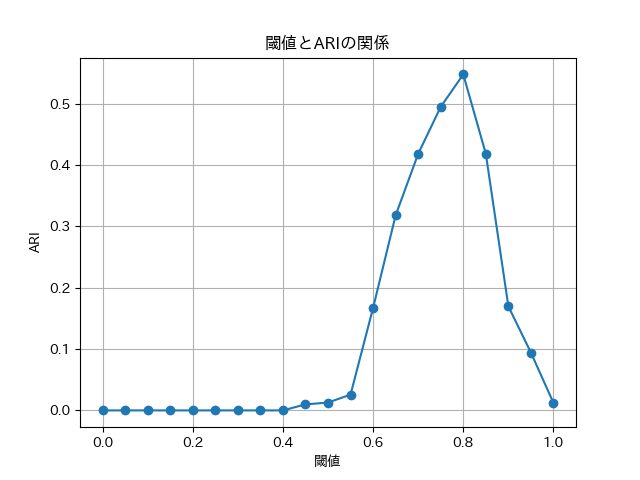
\includegraphics[scale=0.8]
    {contents/images/cw_graph.png}
  \caption{閾値ごとのARIの結果\label{fig:cw_graph}}
\end{figure}
図\ref{fig:cw_graph}から, 閾値が0.8の時にARIが最も高くなることがわかる. したがって本研究では全てのデータのクラスタリングにおいて閾値は0.8に設定して実行した.

そして, 閾値を変更するとその閾値に応じてグラフが作成されるためクラスタ数が変化する. \ref{graph_clustering}項で先述した通り, 閾値が高いほどクラスタの結束力が高まるため閾値を大きくするとクラスタ数が多くなる. 閾値を変化させた際のクラスタ数とARIの関係を図\ref{fig:cw_cluster_graph}に示す.

\begin{figure}[H]
  \centering
  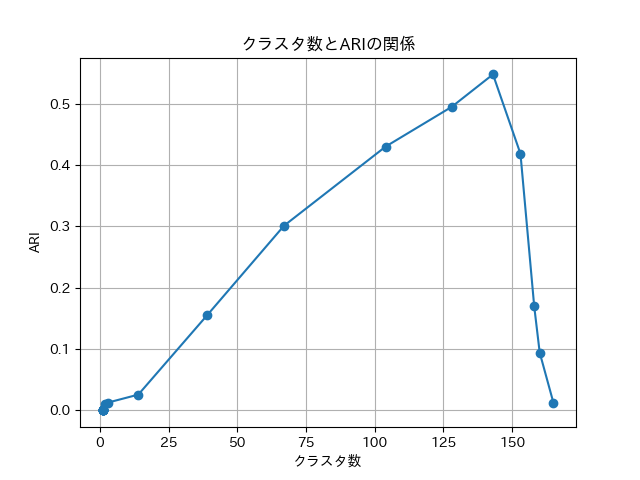
\includegraphics[scale=0.8]
    {contents/images/cw_cluster_graph.png}
  \caption{クラスタ数ごとのARIの結果\label{fig:cw_cluster_graph}}
\end{figure}

図\ref{fig:cw_cluster_graph}から, クラスタ数が143の時にARIが最も高くなることがわかる. 正解データのクラスタ数は123であるため, 正解データよりクラスタ数が約20多くなり, より細かい粒度でのクラスタリングをしていることがわかる.  
ここで, 閾値, クラスタ数, ARIの関係を表\ref{tb:cw_result}に示す. 

\begin{table}[H]
  \caption{閾値, クラスタ数, ARIの関係}
  \label{tb:cw_result}
  \begin{center}
  \begin{tabular}{r|r|r}
    \hline
    閾値&クラスタ数&ARI\\\hline\hline
    0.00&1&0.00\\\hline
    0.05&1&0.00\\\hline
    0.10&1&0.00\\\hline
    0.15&1&0.00\\\hline
    0.20&1&0.00\\\hline
    0.25&1&0.00\\\hline
    0.30&1&0.00\\\hline
    0.35&1&0.00\\\hline
    0.40&1&0.00\\\hline
    0.45&2&0.01\\\hline
    0.50&3&0.01\\\hline
    0.55&14&0.03\\\hline
    0.60&39&0.16\\\hline
    0.65&67&0.30\\\hline
    0.70&104&0.43\\\hline
    0.75&128&0.50\\\hline
    \textbf{0.80}&\textbf{143}&\textbf{0.55}\\\hline
    0.85&153&0.42\\\hline
    0.90&158&0.17\\\hline
    0.95&160&0.09\\\hline
    1.00&165&0.01\\\hline
  \end{tabular}\end{center}
\end{table}

表\ref{tb:cw_result}から, 閾値は0.4以下であると全て同じクラスタとなってしまうことがわかる. 
また, 閾値が0.75の時にクラスタ数が128となっており, 閾値が0.8の場合よりも正解データとのクラスタ数の差が小さい. しかし, 閾値が0.8の方がARIは大きくなる. 


\subsection{他の手法との比較}

K-Means, 階層型クラスタリングは共にクラスタ数を事前に選択する必要があるためクラスタ数をいくつに設定すると最もARIが高くなるか検証した. 
K-Meansにおけるクラスタ数とARIの関係を図\ref{fig:kmeans_graph}, 階層型クラスタリングにおけるクラスタ数とARIの関係を図\ref{fig:agg_graph}にそれぞれ示す.

\begin{figure}[H]
  \centering
  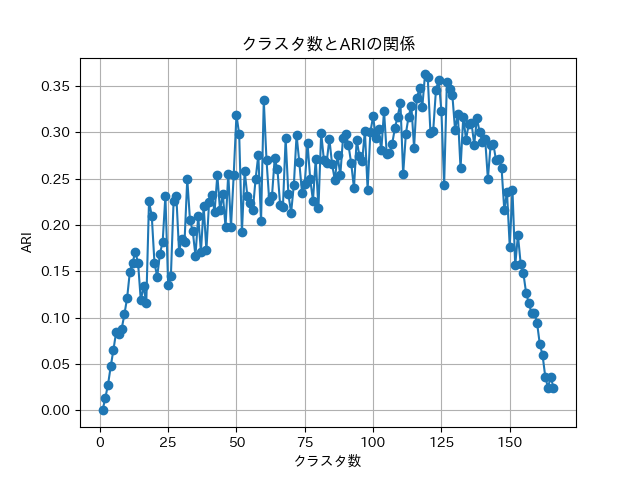
\includegraphics[scale=0.8]
    {contents/images/kmeans_graph.png}
  \caption{K-Meansにおけるクラスタ数ごとのARIの結果\label{fig:kmeans_graph}}
\end{figure}

\begin{figure}[H]
  \centering
  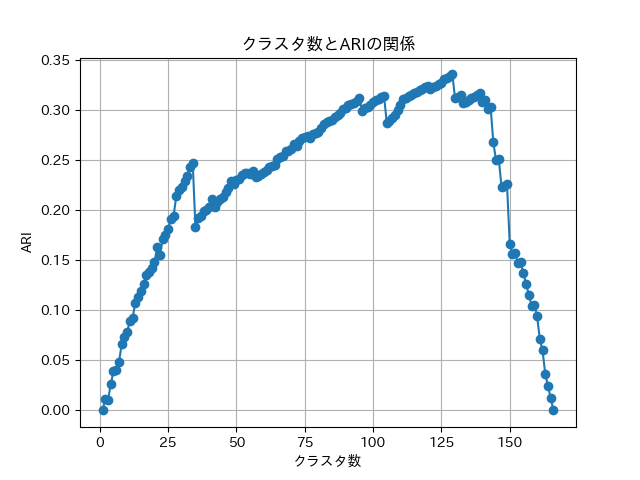
\includegraphics[scale=0.8]
    {contents/images/agg_graph.png}
  \caption{階層型クラスタリングにおけるクラスタ数ごとのARIの結果\label{fig:agg_graph}}
\end{figure}

検証した結果, K-Meansではクラスタ数が119, 階層型クラスタリングではクラスタ数が129の時にそれぞれARIは最も高い値を示した. 次にK-Means, 階層型クラスタリングとChinese WhispersのARIの最大値とその際のクラスタ数を比較した結果が表\ref{tb:two_ari}である. 

\begin{table}[H]
  \caption{3つの手法におけるARI}
  \label{tb:two_ari}
  \begin{center}
  \begin{tabularx}{\linewidth}{X|r|r}
    \hline
    手法&ARIの最大値&クラスタ数\\\hline\hline
    手動&-&123\\\hline
    階層型クラスタリング&0.34&129\\\hline
    K-Means&0.36&119\\\hline
    Chinese Whispers&\textbf{0.55}&143\\\hline
  \end{tabularx}\end{center}
\end{table}

比較した結果, Chinese WhispersのARIの最大値は階層型クラスタリングよりも0.21, K-Meansよりも0.18ほど高いことが示された. また, クラスタ数において, Chinese Whispersは他の手法や正解データと比較するとおよそ20ほど多いことがわかる. 
この結果から, Chinese Whispersは他の手法と比較してより細分化したクラスタリングを行うことがわかる. 

\subsection{総括}
Chinese Whispersで作成されるグラフの閾値について検証した結果, 閾値を0.8としたときに最もARIが高い値を示すことがわかった. 
また, K-Means, 階層型クラスタリング, Chinese Whispersの3つの手法におけるARIの最大値を比較した結果, Chinese Whispersが最もARIが高くなったことから本研究のクラスタリング性能の高さを示すことができた. 

%ーーーーーーーーーーーーーーーーーーーーーーーーーーーー

\section{RQ3:可視化ツールの有用性はどうか}
\subsection{評価方法}
抽出, クラスタリングによって得られた結果を表示する可視化ツールの有用性について示す. 一般的にレビューの閲覧や確認で使用されるGoogle Playストアのレビュー欄と比較して, 本研究で作成した可視化ツールがレビューの分析にどのように役立つのかを記述する. 

\subsection{Google Playストアのレビュー欄}
Google Playストアのレビュー欄は図\ref{fig:google_play}, 図\ref{fig:google_play_graph}のような構成となっている. 

\begin{figure}[H]
  \centering
  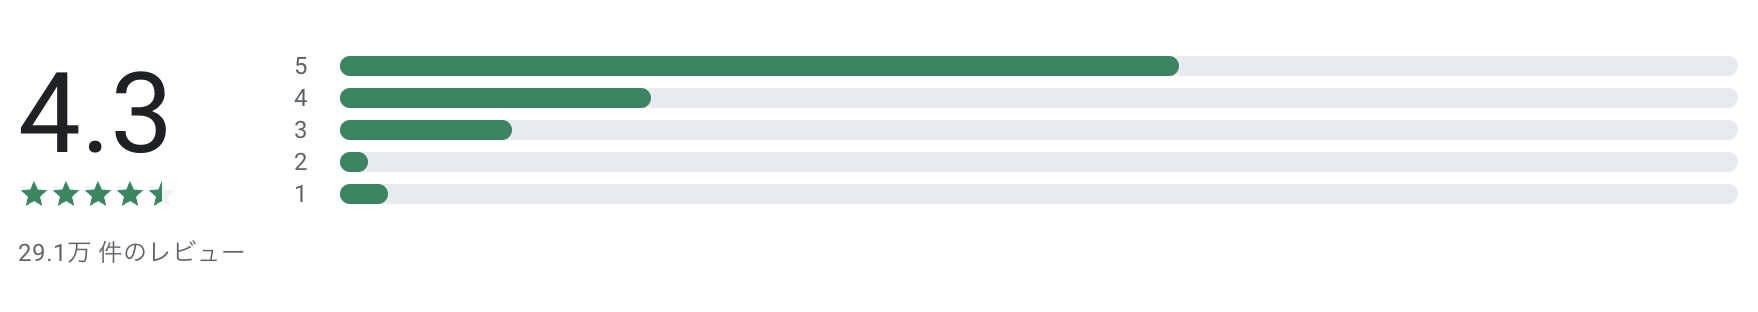
\includegraphics[scale=0.4]
    {contents/images/google_play_graph.png}
  \caption{各評価の数を表すグラフ\label{fig:google_play_graph}}
\end{figure}

\begin{figure}[H]
  \centering
  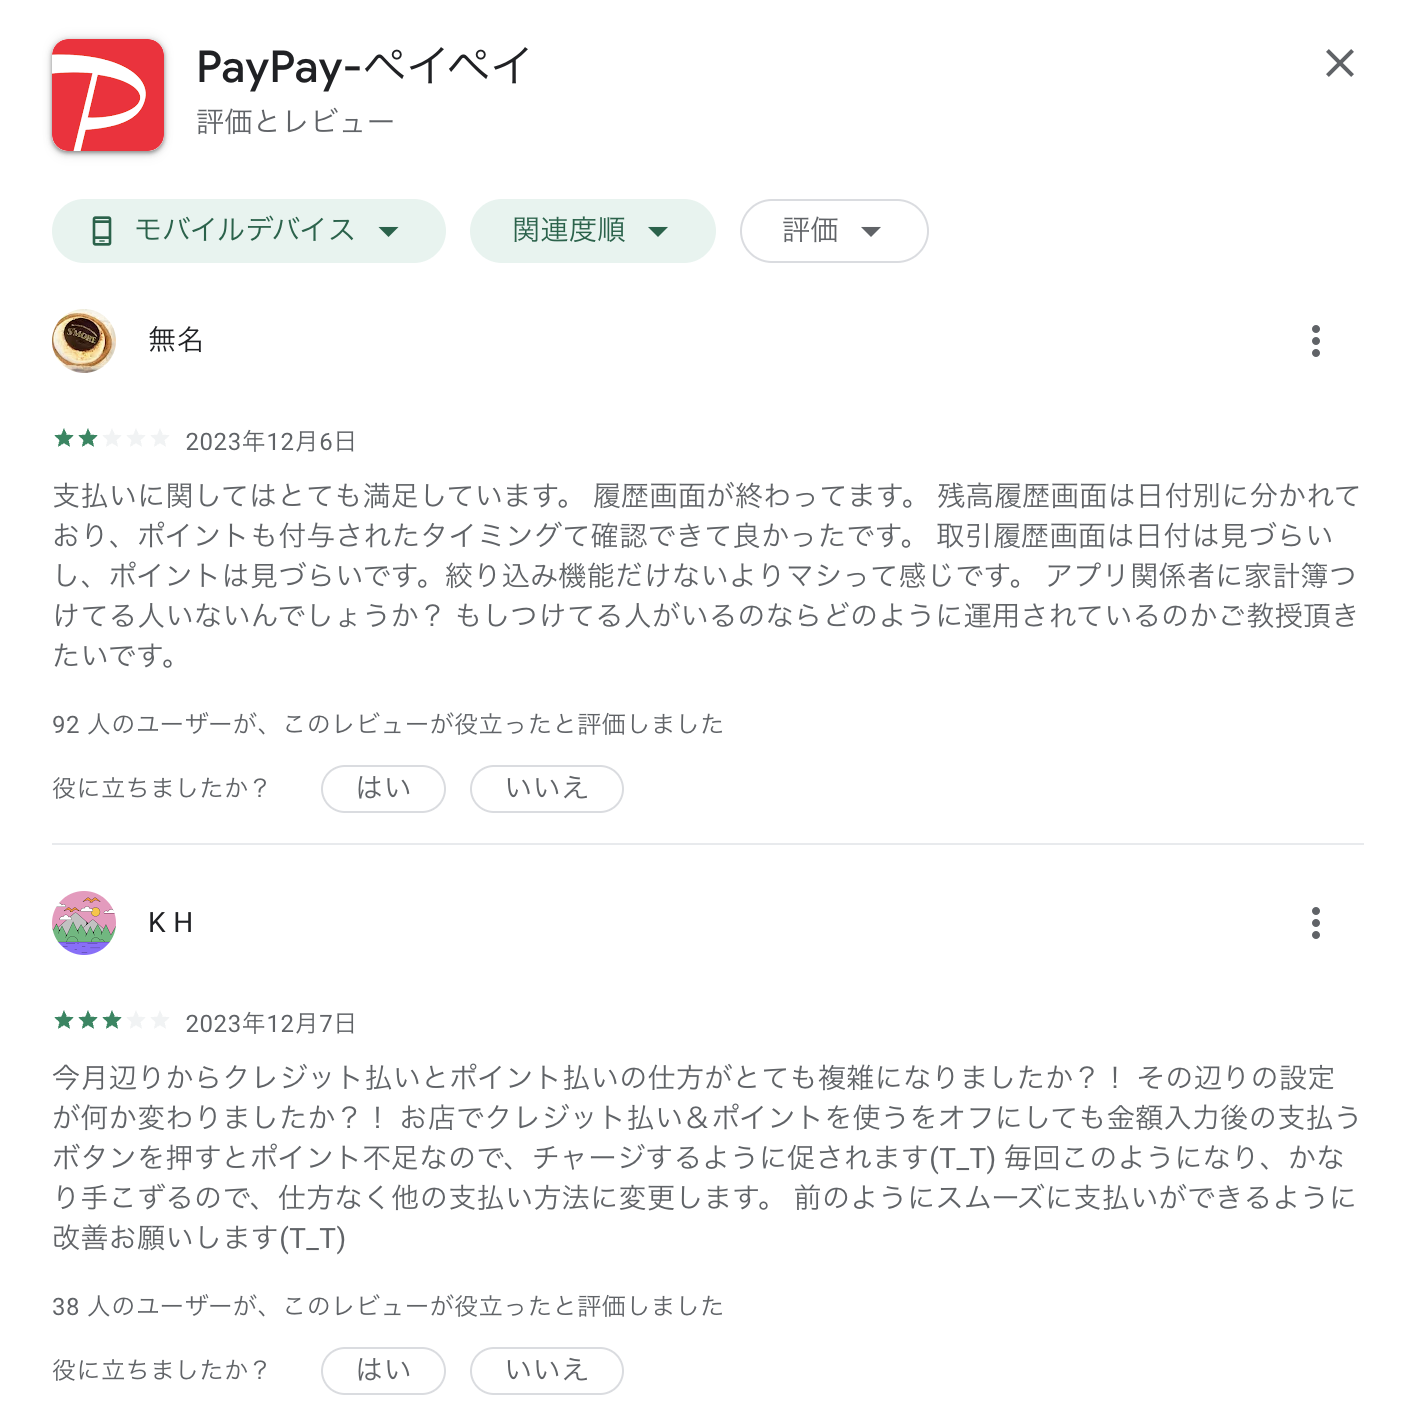
\includegraphics[scale=0.4]
    {contents/images/google_play.png}
  \caption{Google Playストアのレビュー欄\label{fig:google_play}}
\end{figure}

Google Playストアのレビュー欄では評価 (星1〜星5) がそれぞれいくつ付けられているのかを表示するグラフ (図\ref{fig:google_play_graph}) と, 各レビューが記載されている (図\ref{fig:google_play}) . 各レビューには何人のユーザが役に立ったかが記載されており, これによりユーザから見た各レビューの評価がわかる. 
また, 主な機能として評価ごとの絞り込み, 評価や時系列による並び替えがある. 

Google Playストアのレビュー欄と本研究の可視化ツールの違いを示すことで本研究の可視化ツールの有用性を示す. 

\subsection{キーワードと期間の検索}
この可視化ツールではキーワードの検索により特定の機能に関するレビューを絞り込むことができる. また, 期間を絞り込むことにより特定の期間に投稿されたレビューのみを表示することができる.  

この機能は特にアプリのアップデート時に活用できる. アプリのアップデート時に開発者は改善した機能や新しく追加した機能が正常に動いているかどうか, アップデートの前後でレビュー数に変化があるかどうかを確認したい. そのため, この検索機能を用いて分析対象となるレビューを期間とキーワードで絞り込むことで確認するレビュー数を大幅に減らすことができる. 

図\ref{fig:paypay_search}は期間 (2021/10/21〜2021/11/11) ・キーワード (ログイン) で検索した例である. このように, 検索機能を活用して特定の期間や機能に関するレビューのみを表示することが可能となっている. 
\begin{figure}[H]
  \centering
  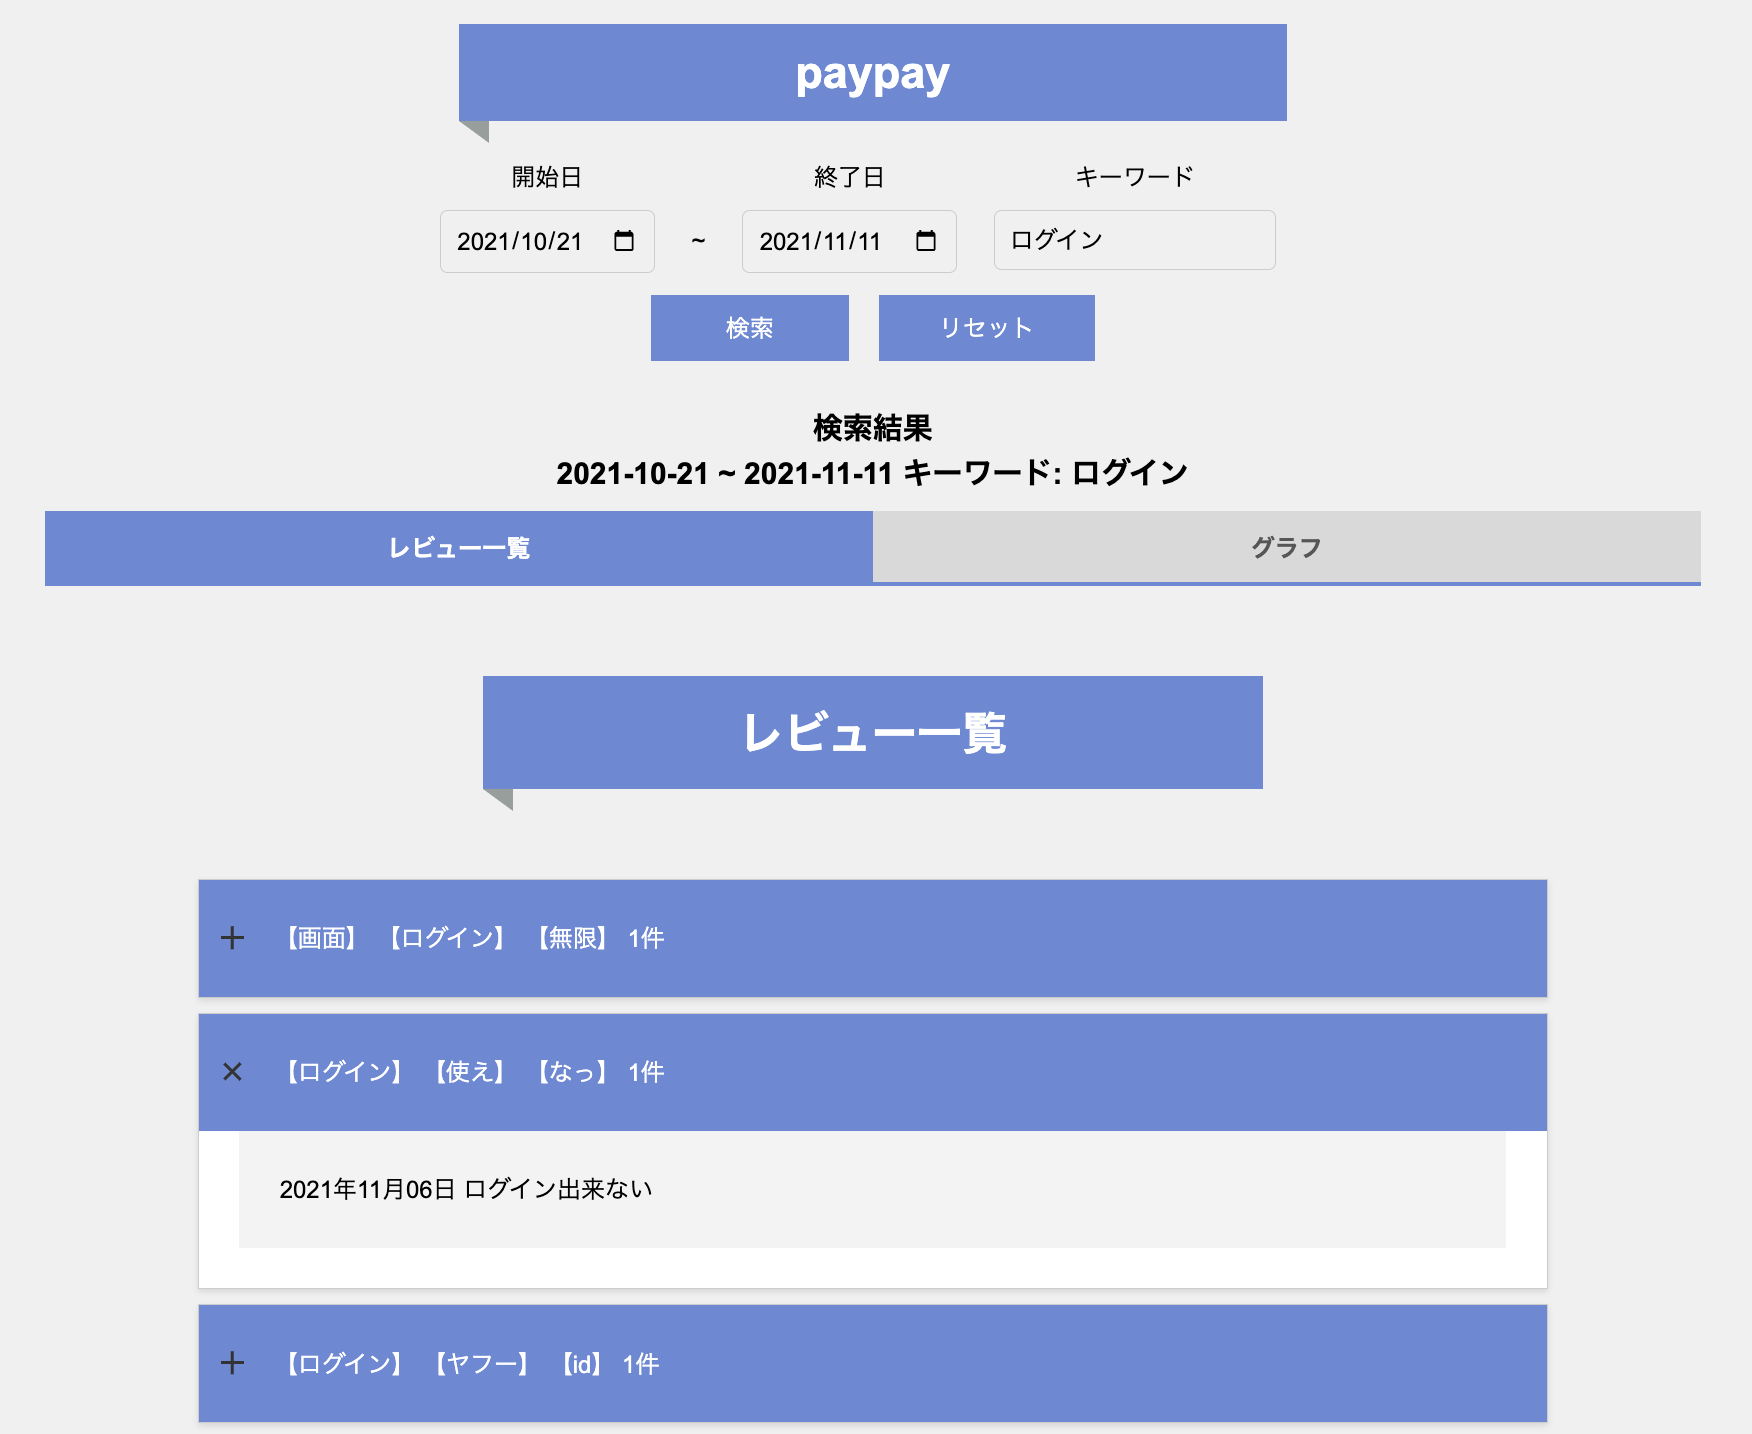
\includegraphics[scale=0.3]
    {contents/images/paypay_search.png}
  \caption{paypayのレビュー検索結果\label{fig:paypay_search}}
\end{figure}

% \subsection{アプリ間のレビュー比較}
% この可視化ツールでは一覧画面にてアプリごとのレビュー数の推移を表示することができる. そのためアプリ間でレビュー数にどのような変化があるのかを1つのグラフで確認することができる. 

% Google Playストアにおける日付とレビュー数の関係を表した折れ線グラフが図\ref{fig:google_graph}である. このグラフは右側にあるアプリ名をタップすることによりグラフ表示のON/OFFが切り替えられるようになっている. 
% また, 検索結果に応じて日付やレビュー数が動的に変更されるようになっている. 

% \begin{figure}[H]
%   \centering
%   \includegraphics[scale=0.3]
%     {contents/images/google_graph.png}
%   \caption{Google Playストアにおける日付とレビュー数の関係\label{fig:google_graph}}
% \end{figure}

% この機能を用いて, 類似した機能を持つアプリがどのような問題を抱えているかを分析することができる. 類似したアプリで見つけられた欠陥は自身の開発しているアプリで同じような欠陥が見つかる可能性がある. 
% したがって開発者はこの可視化ツールで他のアプリのレビューを確認することにより自身の開発に活用することができる. 

\subsection{レビューの分析時間短縮}
Google Playストアのレビュー欄の欠点として, 開発に役立たないレビューが多く存在し, 似たような機能の記述がまとまっていないことが挙げられる. そのため開発者がレビューを分析するのに時間がかかってしまう. 
このような欠点を解消したのが本研究の可視化ツールである. この可視化ツールは開発に役立つレビューかどうかをフィルタリングして類似したレビューをまとめて表示している. そのため開発者はレビューを分析する時間を大幅に短縮できる. 

また, Google Playストアのレビュー欄ではどの期間に多くのレビューが投稿されたかを確認するのに時間がかかる. しかし, 本研究の可視化ツールであれば日ごとのレビュー数の推移をグラフにより表示しているため, どの期間に多くのレビューが書かれているかを確認できる. 
多くのレビューが投稿されている期間が確認できると, その期間に投稿されたレビューを集中的に確認することでアプリの欠陥などを把握することができる. 
このように本研究の可視化ツールを使用することにより, レビューの分析や閲覧にかかる時間を大幅に短縮することが可能となる. 

\subsection{多大な情報量}
本研究の可視化ツールにはGoogle Playストアのレビューだけではなく, Twitterのツイートも表示している. そのためユーザのさまざまな意見を閲覧することができる. 
2021年10月21日から2021年12月15日に取得されたGoogle Playストアのレビュー7,912件とTwitterのツイート1,525,211件のうち, 抽出モデルによって抽出されたキーフレーズの数は表\ref{tb:app_count}となった. 

\begin{table}[H]
  \small
  \caption{抽出されたキーフレーズの数}
  \label{tb:app_count}
  \begin{center}
  \begin{tabularx}{\linewidth}{X|r|r}
    \hline
    アプリ名&Google Playストア&Twitter\\\hline\hline
    にゃんトーク&\textbf{199}&144\\\hline
    スマートニュース&\textbf{615}&134\\\hline
    PayPay&546&\textbf{10,706}\\\hline
    Coke ON&\textbf{1,212}&568\\\hline
    Google Fit&\textbf{570}&307\\\hline
    Simeji&359&\textbf{1,441}\\\hline
    Lemon8&25&\textbf{27}\\\hline
    楽天ペイ&541&\textbf{1,253}\\\hline
    majica&\textbf{1,084}&85\\\hline
    LINE MUSIC&519&\textbf{2,694}\\\hline
    BuzzVideo&146&\textbf{299}\\\hline
    ファミペイ&163&\textbf{314}\\\hline
    CapCut&166&\textbf{261}\\\hline\hline
    合計&6,145&\textbf{18,233}\\\hline
  \end{tabularx}\end{center}
\end{table}

\noindent
表\ref{tb:app_count}からわかるように同一期間で比較した場合, Google PlayストアよりもTwitterの方が抽出されたキーフレーズの数が多いことがわかる. 
この結果からTwitterのツイートは開発者にとって有益な情報を多く含むことがわかる. したがって, Google Playストアのレビューだけでなく, Twitterのツイートを分析対象として, 分析した結果を可視化ツールで表示することは開発者にとって有用であることがわかる. 

\subsection{総括}
本研究で作成された可視化ツールを使用することにより, 開発者がレビューを確認する時間の短縮や効率の向上につながっている. また, Twitterのツイートを分析対象としていることにより提供できる情報量が多いことはこの可視化ツールの大きな特徴である. 
膨大な数が存在するレビューの分析を効率化させることは開発者にとって1つの課題であるため本研究の可視化ツールは非常に有用であると考えられる. 

\section{妥当性の脅威}
\subsection{対象アプリ}
本研究の対象アプリはデータ取得の問題により先行研究のアプリに合わせている. アプリの選択はカテゴリーについて考慮されていないため, 様々なカテゴリーのアプリにおける提案手法の有効性は確保されていない. 
したがって, 様々なカテゴリーに属する多くのアプリのレビューデータに提案手法を実行して, 有効性を確認する必要がある. 

\subsection{トレーニングデータ}
本研究では情報工学科の学生2人により10,000件のレビューからトレーニングデータを作成した. RQ1でも述べたように, このトレーニングデータの精度には改善の余地がある. 
トレーニングデータの精度を向上させるために, アプリの開発者などレビューに関する専門的知識を持つ人がトレーニングデータを作成する, トレーニングデータを作成する人数を増やして議論するなど工夫が必要である. 
また, 本研究ではトレーニングデータの数を増やすことにより抽出の精度が上がるかどうかを検証していない. そのため, データ数と自動抽出精度の関係性に関して更なる調査が必要である. 

\subsection{自動抽出とクラスタリングの関係性}
提案手法では自動抽出したキーフレーズを意味に応じてクラスタリングしている. したがって, クラスタリングの精度は自動抽出の精度に依存する. 
RQ1の結果から自動抽出には改善の余地が見られるため, クラスタリングした際に精度の悪さが蓄積する危険性がある. クラスタリングの精度向上には自動抽出の精度向上が必要であると考えられる. 